\documentclass[12pt]{report}

\usepackage[utf8]{inputenc}
\usepackage{parskip}
\usepackage{graphicx}

\title{Assignment 1}
\author{Lasse Berglund : 48-159707}
\date{\today}

% User ID student
% Password biznet

\begin{document}
\maketitle
\section*{1}
Plotted with Wolfram Alpha:

\subsection*{(a)}
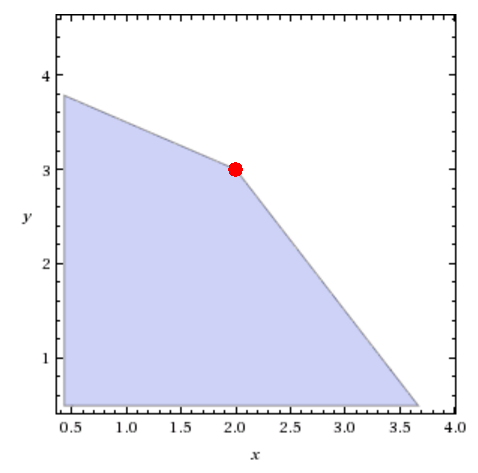
\includegraphics[scale=0.35]{1_a.png}\\ 
\subsection*{(b)}
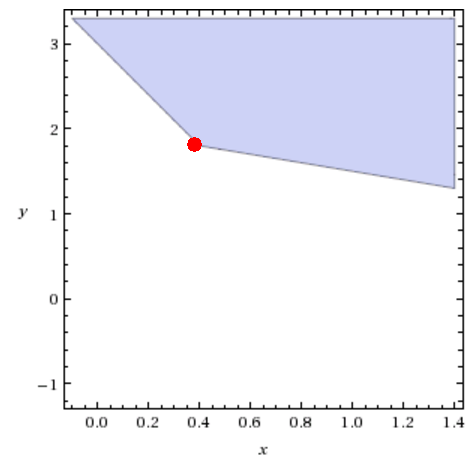
\includegraphics[scale=0.35]{1_b.png}

\newpage

\section*{2}
\subsection*{(a)}
Where $x$ is the amount of raw carrots, $y$ is the amount white cabbage, and $z$ is the amount of pickled cucumber. \\ \\
\textbf{Minimize}\\
  $0.75 x + 0.5 y + 0.15 z$\\
\textbf{subject to:}\\
  $c_1: 35 x + 0.5 y + 0.5 z \ge 0.5 $ \\
  $c_2: 60 x + 300 y + 10 z \ge 15 $ \\
  $c_3: 30 x + 20 y + 10 z \ge 4 $ \\

\subsection*{(b)}
Using this program in SCIP:
\begin{verbatim}
minimize
  0.75 x + 0.5 y + 0.15 z
subject to
  c1: 35 x + 0.5 y + 0.5 z >= 0.5
  c2: 60 x + 300 y + 10 z >= 15
  c3: 30 x + 20 y + 10 z >= 4
end
\end{verbatim}
I got the following results: \\ \\
objective value: $0.0705$\\
x $0.009526$   (obj:0.75) \\
y $0.038265$   (obj:0.5) \\
z $0.294891$   (obj:0.15)


\section*{3}
\subsection*{(a)}
Again plotted using Wolfram Alpha.

\includegraphics[scale=0.6]{3_a}

I do not feel like I can guess the optimal solution from this region.

\subsection*{(b)}

I formulated the problem as the following program in SCIP.

I replaced the expression $|x_2-10|$ in the objective function with the new variable $x_3$ and added constraints to ensure that no information was lost. Additionally I added four constraints to remove the two absolute values in the original constraint.

\begin{verbatim}
minimize
  2x1 + 3x3
subject to
  x2 - x3 <= 10 
  -x2 - x3 <= -10
  x1 + 2 + x2 <= 5
  x1 + 2 - x2 <= 5
  -x1 - 2 + x2 <= 5
  -x1 - 2 - x2 <= 5
end
\end{verbatim}

The solution given as optimal by SCIP was: \\
objective value: $22.5$\\
$x_1: 0$ \\
$x_2: 2.5$ \\
$x_3: 7.5$ \\



\section*{4}
In my personal life, my biggest optimization problem is related to scheduling. Deciding when to work on what, trying to get as much work as possible in the shortest amount of time. Obviously it depends on a lot of factors.

An optimization problem that affects most people in Tokyo is the train system. Obviously the companies want to transport as many people as they can, using as few trains as possible (to keep costs down).

\end{document}